\subsection{Trigonometric Functions}

\subsubsection{Angles in Standard Position}
Angles are often interpreted as rotations of a line or ray. The starting position is called the initial arm (usually this is the x-axis) and the final position is the terminal arm.\\
If the rotation is counterclockwise, we consider it to be positive. If the rotation is clockwise, we consider it to be negative.\\
The angle $\theta$ is the total rotation from the x-axis. The reference angle, $\theta_R$, is the absolute value of the angle the line makes with the x-axis.\\
\centerline{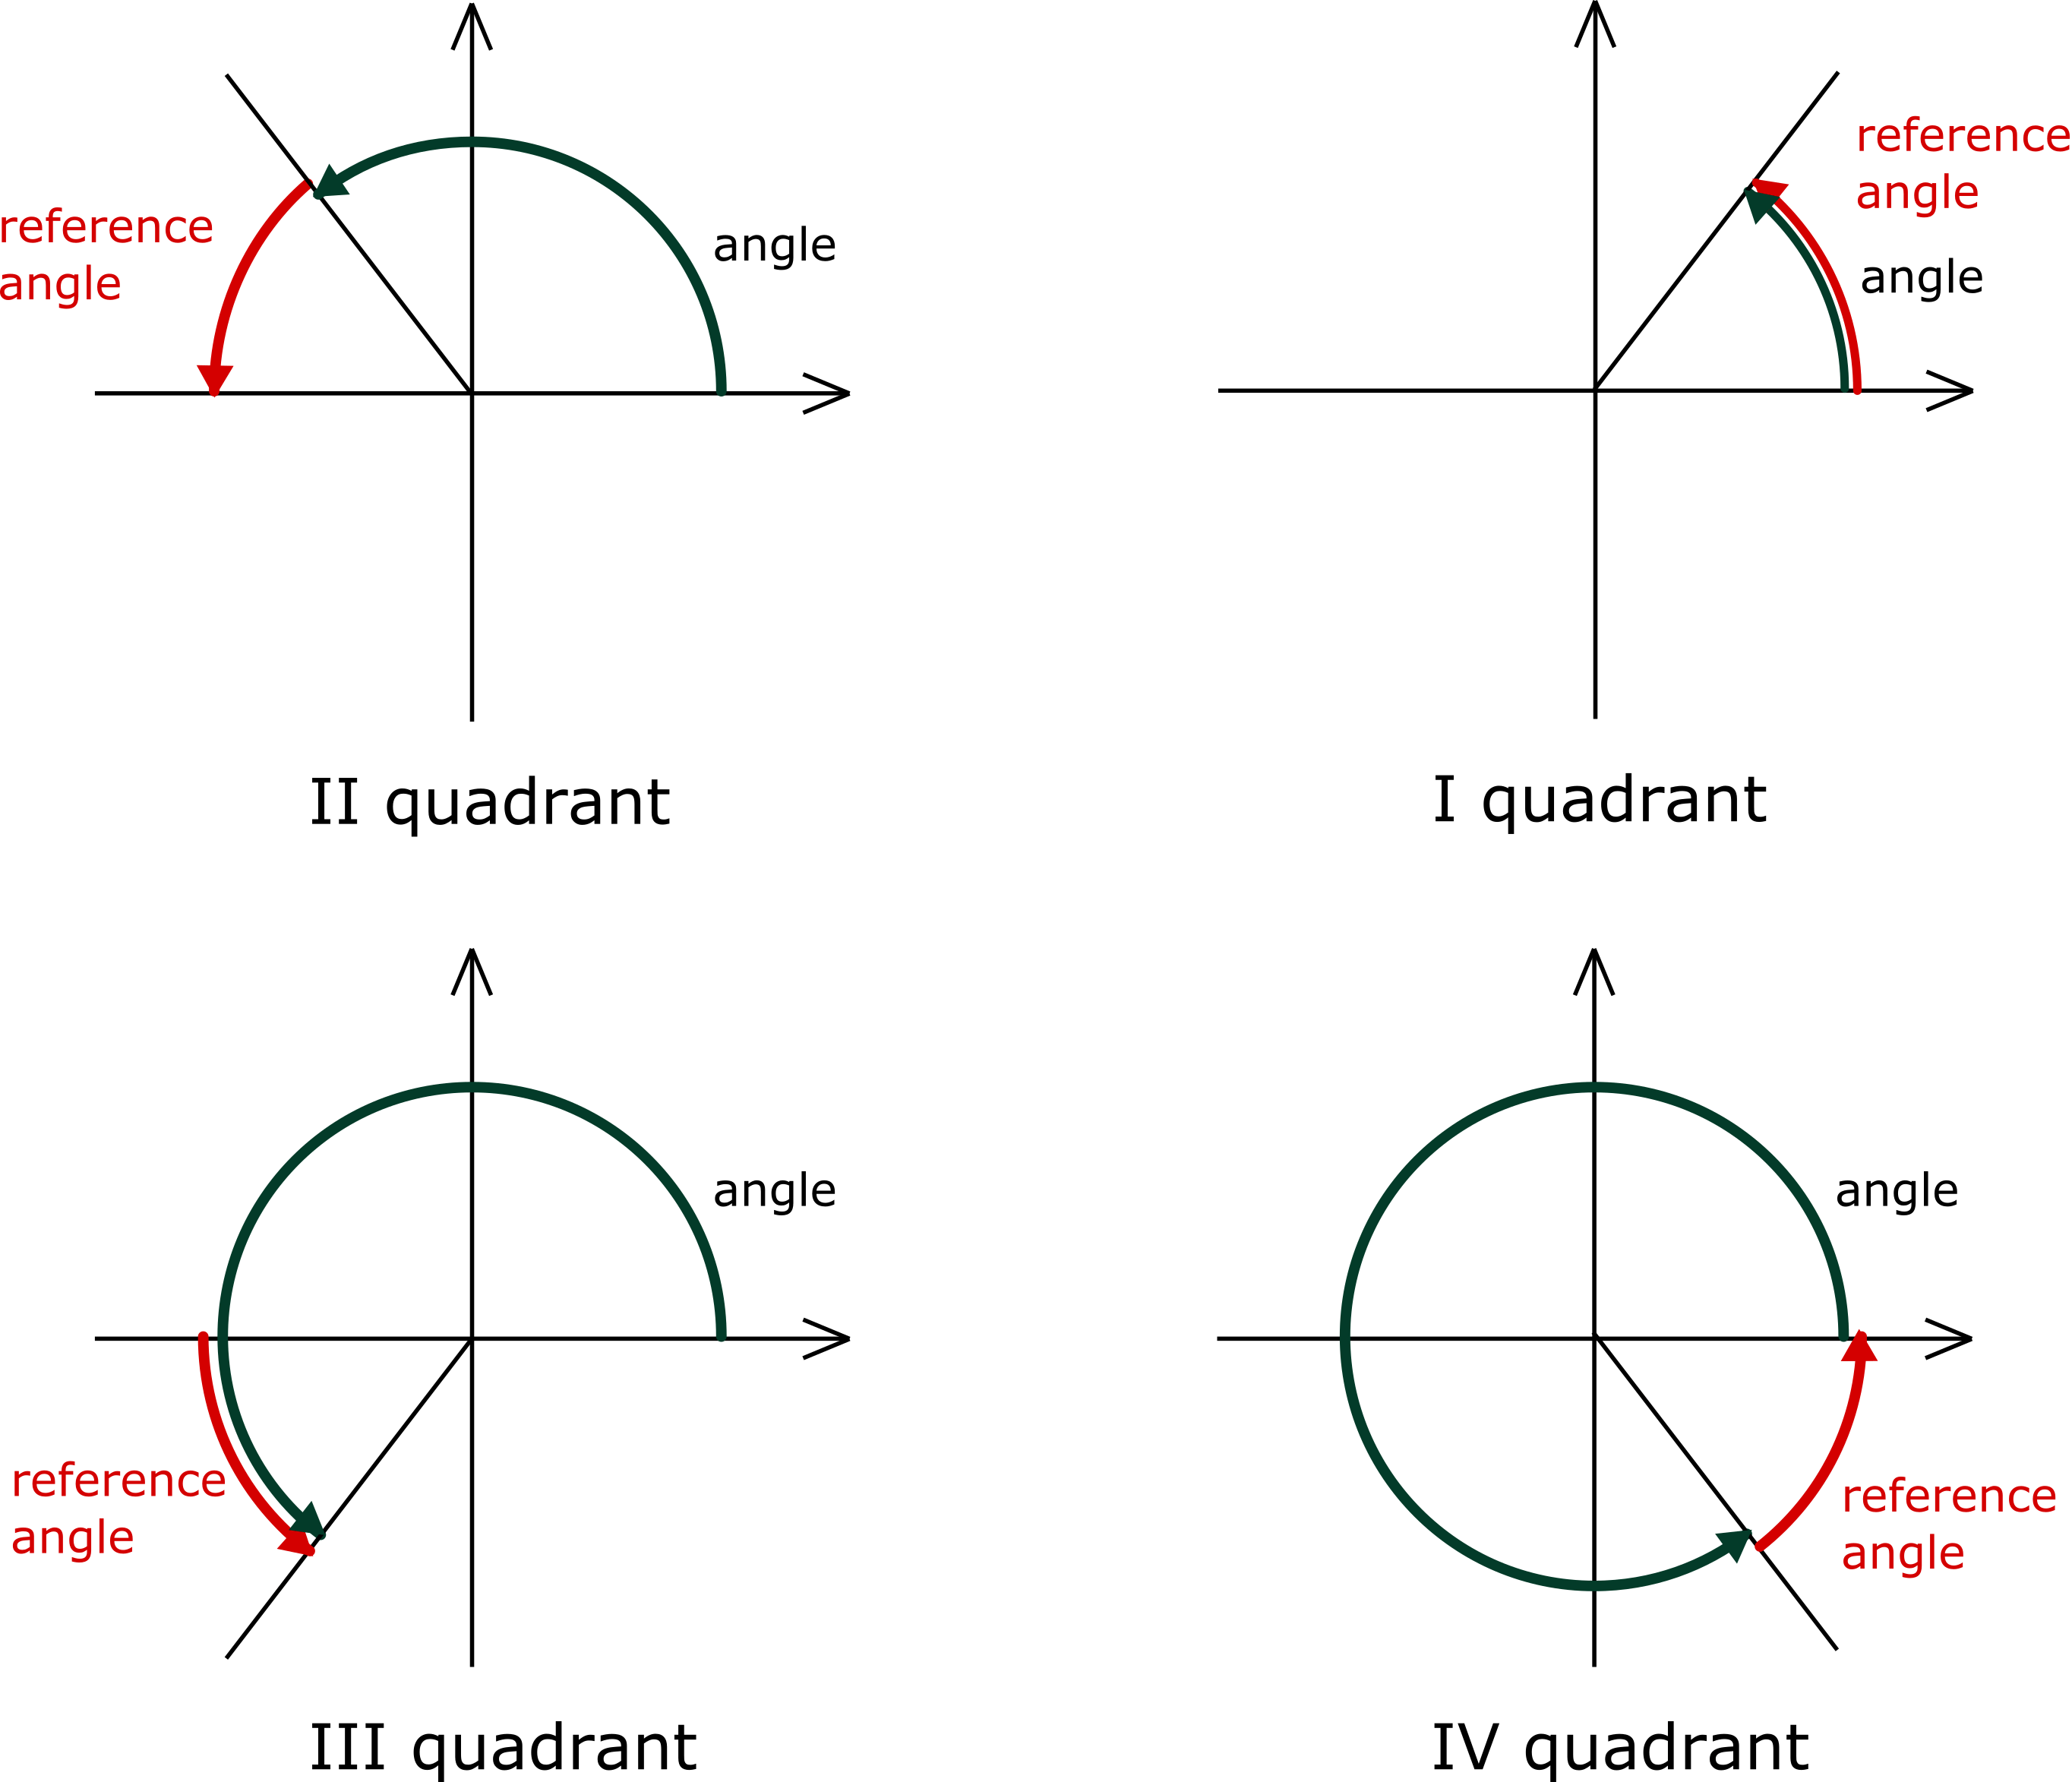
\includegraphics[scale=0.13]{Images/PreCalcPictures/ReferenceAngle.png}}
If we draw a line from the origin to a point $(x,y)$, we can form a triangle and express trig ratios in terms of $x$ and $y$.
$$\sin\theta=\frac{y}{r},\,\cos\theta=\frac{x}{r},\,\tan\theta=\frac{y}{x}$$
Depending which quadrant we are in, these ratios will either be positive or negative.
\begin{align*}
    &\mathrm{QI:}\,\sin\theta>0,\,\cos\theta>0,\,\tan\theta>0\\
    &\mathrm{QII:}\,\sin\theta>0,\,\cos\theta<0,\,\tan\theta<0\\
    &\mathrm{QIII:}\,\sin\theta<0,\,\cos\theta<0,\,\tan\theta>0\\
    &\mathrm{QIV:}\,\sin\theta<0,\,\cos\theta>0,\,\tan\theta<0
\end{align*}

\subsubsection{Primary Trigonometric Functions}
To further simplify, these trig ratios, we can define the unit circle: a circle with radius 1 centered at the origin. This allows us to express any point on the circle in terms of sines and cosines.\\
$(x,y)=(\cos\theta,\sin\theta)$\\
In doing this, we can define $\sin\theta$ to be the height of the circle and $\cos\theta$ as the horizontal component of the circle.\\
\centerline{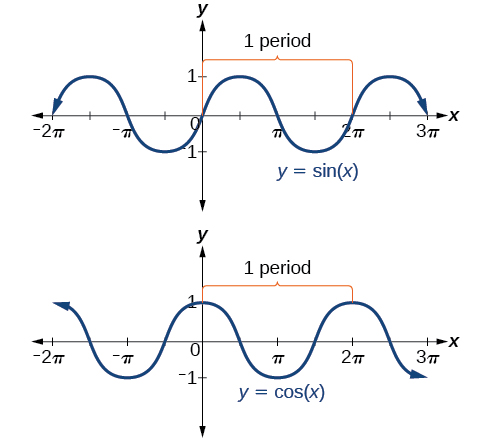
\includegraphics[scale=1.2]{Images/PreCalcPictures/SinxandCosx.jpg}}
Both functions are called sinusoidal curves because they resemble waves. The only difference between the two is that they are shifted over from another by $\frac{\pi}{2}$. They share a common domain and have a range of $y\in[-1,1]$\\
$y=\sin x$ has x-intercepts every $n\pi,\,n\in\mathbb{Z}$\\
$y=\cos x$ has intercepts every $\frac{\pi}{2}+n\pi,\, n\in \mathbb{Z}$\\
The equations in general form are
$$y=a\sin\left(\frac{1}{b}(x-c)\right)+d\text{ and }y=a\cos\left(\frac{1}{b}(x-c)\right)+d$$
Definitions:
\begin{itemize}
    \item Periodic Function: A function that repeats in a regular pattern over a regular interval
    \item Sinusoidal Curve: Curves whose graphs look like waves
    \item Cycle: Portion of a graph to the point it repeats
    \item Period: Length across the x-axis for one cycle
    \item Amplitude: Half the distance between the minimum and maximum values
    \item $d$ is vertical displacement
    \item $c$ is phase shift
    \item $a$ is amplitude
    \item $b$ is change in period
\end{itemize}
Sine and cosine have periods of $2\pi b$.\\ Tangent is defined as $\tan x=\dfrac{\sin x}{\cos x}$ and has a period of $\pi b$\\
\centerline{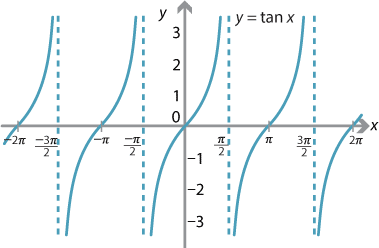
\includegraphics[scale=0.9]{Images/PreCalcPictures/tanx.png}}
$\tan x$ has vertical asymptotes every $x=\frac{\pi}{2}+n\pi,\,n\in\mathbb{Z}$ and x-intercepts every $\pi n,\,n\in\mathbb{Z}$

\subsubsection{Reciprocal Trigonometric Functions}
The reiprocals of trig functions are defined as
$$\csc\theta = \frac{1}{\sin\theta},\,\sec\theta=\frac{1}{\cos\theta},\,\cot\theta=\frac{1}{\tan\theta}=\frac{\cos\theta}{\sin\theta}$$
They will have vertical asymptotes any place where the original function had a zero and they will have x-intercepts any place where the original function had a vertical asymptote.\\
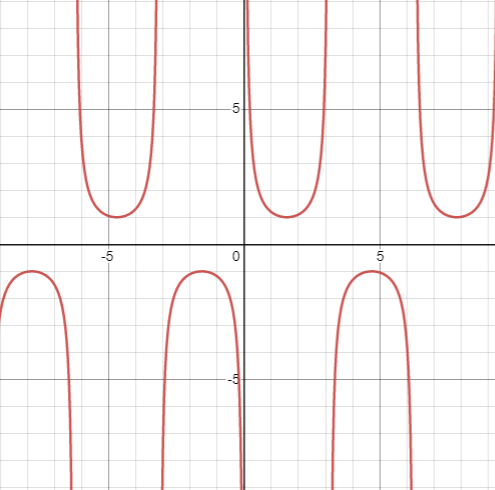
\includegraphics[scale=0.4]{Images/PreCalcPictures/Cscx.png}\
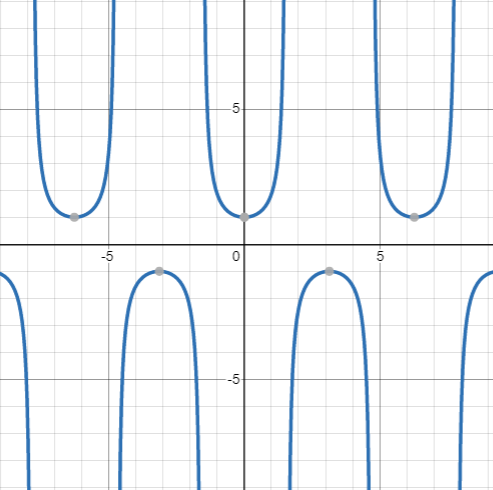
\includegraphics[scale=0.4]{Images/PreCalcPictures/Secx.png}\
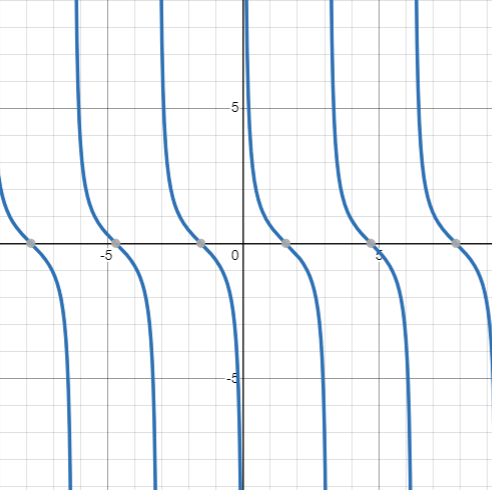
\includegraphics[scale=0.4]{Images/PreCalcPictures/Cotx.png}\\
Shown in order of $\csc x,\,\sec x,\,\cot x$

\subsubsection{Trigonometric Identities}
Pythagorean Identities:\\
These identities can be derived from the unit circle from where $x^2+y^2=1$ and $\cos\theta = x$ and $\sin\theta=y$ so we get
$$\sin^2\theta+\cos^2\theta=1$$
By dividing by $\sin^2\theta$ we get
$$1+\cot^2\theta=\csc^2\theta$$
By dividing by $\cos^2\theta$ we get 
$$\tan^2\theta+1=\sec^2\theta$$
Even-Odd Identities:
\begin{align*}
    \sin(-\theta)&=-\sin\theta\\
    \csc(-\theta)&=-\csc\theta\\
    \tan(-\theta)&=-\tan\theta\\
    \cot(-\theta)&=-\cot\theta\\
    \cos(-\theta)&=\cos\theta\\
    \sec(-\theta)&=\sec\theta
\end{align*}
Co-Function Identities:
\begin{align*}
    \sin\left(\frac{\pi}{2}-\theta\right)&=\cos\theta\\
    \cos\left(\frac{\pi}{2}-\theta\right)&=\sin\theta\\
    \csc\left(\frac{\pi}{2}-\theta\right)&=\sec\theta\\
    \sec\left(\frac{\pi}{2}-\theta\right)&=\csc\theta\\
    \tan\left(\frac{\pi}{2}-\theta\right)&=\cot\theta\\
    \cot\left(\frac{\pi}{2}-\theta\right)&=\tan\theta
\end{align*}
Sum-Difference Identities:
\begin{align*}
    \sin(A\pm B)&=\sin A\cos B\pm \cos A\sin B\\
    \cos(A\pm B)&=\cos A\cos B\mp \sin A\sin B\\
    \tan(A\pm B)&=\frac{\tan A\pm \tan B}{1\mp\tan A\tan B}
\end{align*}
Double Angle Formulas:\\
These are derived from the sum-difference identities.
\begin{align*}
    \sin(2\theta)&=2\sin\theta\cos\theta\\
    \cos(2\theta)&=\cos^2\theta-\sin^2\theta\\
    &=2\cos^2\theta-1\\
    &=1-2\sin^2\theta\\
    \tan(2\theta)&=\frac{2\tan\theta}{1-\tan^2\theta}
\end{align*}
Power Reducing Formulas:
These are derived from the double angle formulas.
\begin{align*}
    \sin^2\theta&=\frac{1-\cos(2\theta)}{2}\\
    \cos^2\theta&=\frac{1+\cos(2\theta)}{2}\\
    \tan^2\theta&=\frac{1-\cos(2\theta)}{1+\cos(2\theta)}
\end{align*}
Sum to Product Formulas:
\begin{align*}
    \sin A+\sin B&=2\sin\left(\frac{A+B}{2}\right)\cos\left(\frac{A-B}{2}\right)\\
    \sin A-\sin B&=2\cos\left(\frac{A+B}{2}\right)\sin\left(\frac{A-B}{2}\right)\\
    \cos A+\cos B&=2\cos\left(\frac{A+B}{2}\right)\cos\left(\frac{A-B}{2}\right)\\
    \cos A-\cos B&=-2\sin\left(\frac{A+B}{2}\right)\sin\left(\frac{A-B}{2}\right)
\end{align*}
Product to Sum Formulas:
\begin{align*}
    \sin A\sin B&=\frac{1}{2}(\cos(A-B)-\cos(A+B))\\
    \sin A\cos B&=\frac{1}{2}(\sin(A+B)+\sin(A-B))\\
    \cos A\cos B&=\frac{1}{2}(\cos(A-B)+\cos(A+B))
\end{align*}
\\
Trig Proofs:\\
Ex: Prove the following:
\begin{align*}
    \tan x\sin x&=\sec x-\cos x\\
    &=\frac{1}{\cos x}-\cos x\left(\frac{\cos x}{\cos x}\right)\\
    &=\frac{1}{\cos x}-\frac{\cos^2x}{\cos x}\\
    &=\frac{1-\cos^2x}{\cos x}\\
    &=\frac{\sin^2x}{\cos x}\\
    &=\tan x\sin x\\
    &\text{Q.E.D.}
\end{align*}
\begin{align*}
    \text{Ex2: }2\cos A\sin B&=\sin(A+B)-\sin(A-B)\\
    &=\sin A\cos B+\sin B\cos A-(\sin A\cos B-\sin B\cos A)\\
    &=\sin B\cos A+\sin B\cos A\\
    &=2\cos A\sin B\\
    &\text{Q.E.D.}
\end{align*}

\subsubsection{Solving Trigonometric Equations}
To solve a trig equation, we want to use trig identities to express the equation as a single term.\\
\begin{align*}
    \text{Ex: }&\cos(2x)-\cos x=0\\
    &2\cos^2x-1-\cos x=0\\
    &(2\cos x+1)(\cos x-1)=0\\
    &\Ra\cos x=\left\{-\frac{1}{2},1\right\}\\
    &x_R=\pi-\frac{\pi}{3}=\frac{2\pi}{3}\\
    &x_R=\pi+\frac{\pi}{3}=\frac{4\pi}{3}\\
    &x_R=0\\
    &\Ra x=\left\{0,\frac{2\pi}{3},\frac{4\pi}{3}\right\}+2\pi n,\,n\in\mathbb{Z}
\end{align*}
\begin{align*}
    \text{Ex2: }&3\sqrt{3}\sin(3x)-3\cos(3x)=3\sqrt{3}\\
    &3\sqrt{3}\sin(3x)=3\sqrt{3}+3\cos(3x)\\
    &27\sin^2(3x)=27+18\sqrt{3}\cos(3x)+9\cos^2(3x)\\
    &3(1-\cos^2(3x))=3+2\sqrt{3}\cos(3x)+\cos^2(3x)\\
    &3-3\cos^2(3x)=3+2\sqrt{3}\cos(3x)+\cos^2(3x)\\
    &4\cos^2(3x)+2\sqrt{3}\cos(3x)=0\\
    &\cos(3x)(4\cos(3x)+2\sqrt{3})=0\\
    &\cos(3x)=0\Ra3x=\left\{\frac{\pi}{2},\frac{3\pi}{2}\right\}+2\pi n,\,n\in\mathbb{Z}\\
    &x=\left\{\frac{\pi}{6},\frac{\pi}{2}\right\}+\frac{2\pi}{3}n,\,n\in\mathbb{Z}\\
    &4\cos(3x)+2\sqrt{3}=0\Ra\cos(3x)=\frac{\sqrt{3}}{2}\Ra3x=\left\{\frac{5\pi}{6},\frac{7\pi}{6}\right\}+2\pi n,\,n\in\mathbb{Z}\\
    &x=\left\{\frac{5\pi}{18},\frac{7\pi}{18}\right\}+\frac{2\pi}{3}n,\,n\in\mathbb{Z}\\
    &\text{Because we squared both sides we may have introduced extraneous roots.}\\
    &\text{To check this, we can plug in the values or solve for the $\sin x$ case}\\
    &\text{and take the $x$ values that satisfy both.}\\
    &3\sqrt{3}\sin(3x)-3\cos(3x)=3\sqrt{3}\\
    &3\sqrt{3}\sin(3x)-3\sqrt{3}=3\cos(3x)\\
    &27\sin^2(3x)-54\sin(3x)+27=9(1-\sin^2(3x))\\
    &3\sin^2(3x)-6\sin(3x)+3=1-\sin^2(3x)\\
    &4\sin^2(3x)-6\sin(3x)+2=0\\
    &\sin(3x)=\frac{1}{2}\Ra3x=\left\{\frac{\pi}{6},\frac{5\pi}{6}\right\}+2\pi n,\,n\in\mathbb{Z}\\
    &\sin(3x)=1\Ra3x=\frac{\pi}{2}+2\pi n,\,n\in\mathbb{Z}\\
    &x=\left\{\frac{\pi}{18},\frac{\pi}{6},\frac{5\pi}{18}\right\}+\frac{2\pi}{3}n,\,n\in\mathbb{Z}\\
    &\therefore\,x=\left\{\frac{\pi}{6},\frac{5\pi}{18}\right\}+\frac{2\pi}{3}n,\,n\in\mathbb{Z}
\end{align*}
\subsubsection{Inverse Trigonometric Functions}
If we take the inverse of a trigonometric function, it would not pass the vertical line test and would not be a function. To get around this, we need to restrict the domain in which we take the inverse.\\
The value from the appropriate range that an inverse function returns is called the principal value of the function.\\
Graphs:\\
\centerline{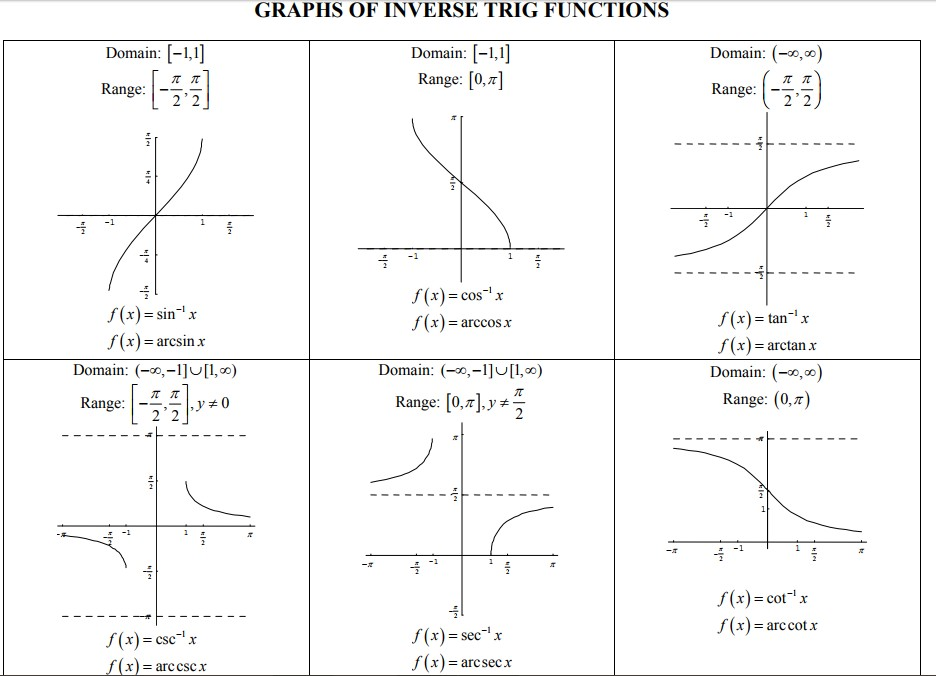
\includegraphics[scale=0.5]{Images/PreCalcPictures/InverseTrigGraphs.png}}

Identities:
\begin{align*}
    &\text{even/odd: }\\
    &\arcsin (-x)=-\arcsin x\\
    &\arccos(-x)=\pi-\arccos x\\
    &\arctan(-x)=-\arctan x\\
    &\arccot(-x)=\pi-\arccot x\\
    &\arccsc(-x)=-\arccsc x\\
    &\arcsec(-x)=\pi-\arcsec x\\
    &\text{Reciprocal:}\\
    &\arcsec x=\arccos\left(\frac{1}{x}\right)\\
    &\arccsc x=\arcsin\left(\frac{1}{x}\right)\\
    &\arccot x=\displaystyle{\left\{\begin{matrix}
    \arctan\left(\frac{1}{x}\right)\text{ if }x\geq 0\\
    \pi+\arctan\left(\frac{1}{x}\right)\text{ if }x<0
    \end{matrix}\right.}\\
    &\arccot x=\frac{\pi}{2}-\arctan x
\end{align*}
Because of the restricted domain, we need to be careful with inverse trig functions.\\
Ex: $\arcsin(\sin(\pi))=\arcsin(0)=0$\\
While $\sin(\arcsin(\pi))$ is undefined.\\
To get around this, we can add or subtract increments of $2\pi$ to get our value within the appropriate range.\\
Ex2: $\arcsin\left(\sin\left(\frac{13\pi}{3}\right)\right)=\arcsin\left(\sin\left(\frac{\pi}{3}\right)\right)=\frac{\pi}{3}$\\
For more complicated examples, we can visualise it with a triangle.\\
Ex3: $\cos(\arcsin x)$\\
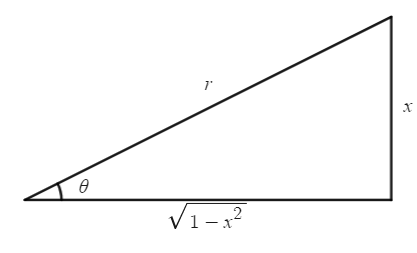
\includegraphics[scale=0.5]{Images/PreCalcPictures/TriangleInvTrig.png}
\begin{align*}
    &\text{let }\theta=\arcsin x\Ra x=\sin\theta\\
    &\Ra\cos\theta=\sqrt{1-x^2}\\
    &\cos(\arcsin x)=\sqrt{1-x^2}
\end{align*}